\documentclass[tikz,border=9pt]{standalone}
\usepackage{amsmath,amssymb}
\usetikzlibrary{arrows.meta,positioning,calc}
\begin{document}
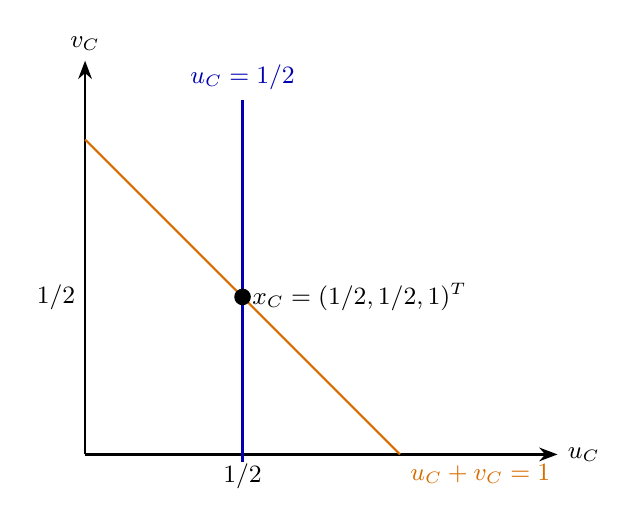
\begin{tikzpicture}[font=\small,arr/.style={-{Stealth},thick},box/.style={draw=blue!55!black,rounded corners,fill=blue!4,align=center,text width=2.9cm,minimum height=1.05cm}]

\draw[arr] (0,0)--(6,0) node[right]{$u_C$};\draw[arr] (0,0)--(0,5) node[above]{$v_C$};
\draw[thick,blue!70!black] (2,-.1)--(2,4.5) node[above]{$u_C=1/2$};
\draw[thick,orange!85!black] (0,4)--(4,0) node[below right]{$u_C+v_C=1$};
\fill (2,2) circle(3pt) node[right]{$x_C=(1/2,1/2,1)^T$};
\node[below] at (2,0){$1/2$};\node[left] at (0,2){$1/2$};

\end{tikzpicture}
\end{document}
